\documentclass[12pt]{article}
\usepackage{graphicx}

\begin{document}
\section{Index of Formula}
{\ref{eq1}} is a binary equation.

{\ref{eq2}} is a binary quadratic equation.
\begin{equation}
    x + y = 2 \label{eq1}
\end{equation}

\begin{equation}
    x^{2} + y^{2} = 2 \label{eq2}
\end{equation}

\section{Index of Figure}
Figure {\ref{kid}} is a photo of a kid.
\begin{figure}[h]
    \centering
    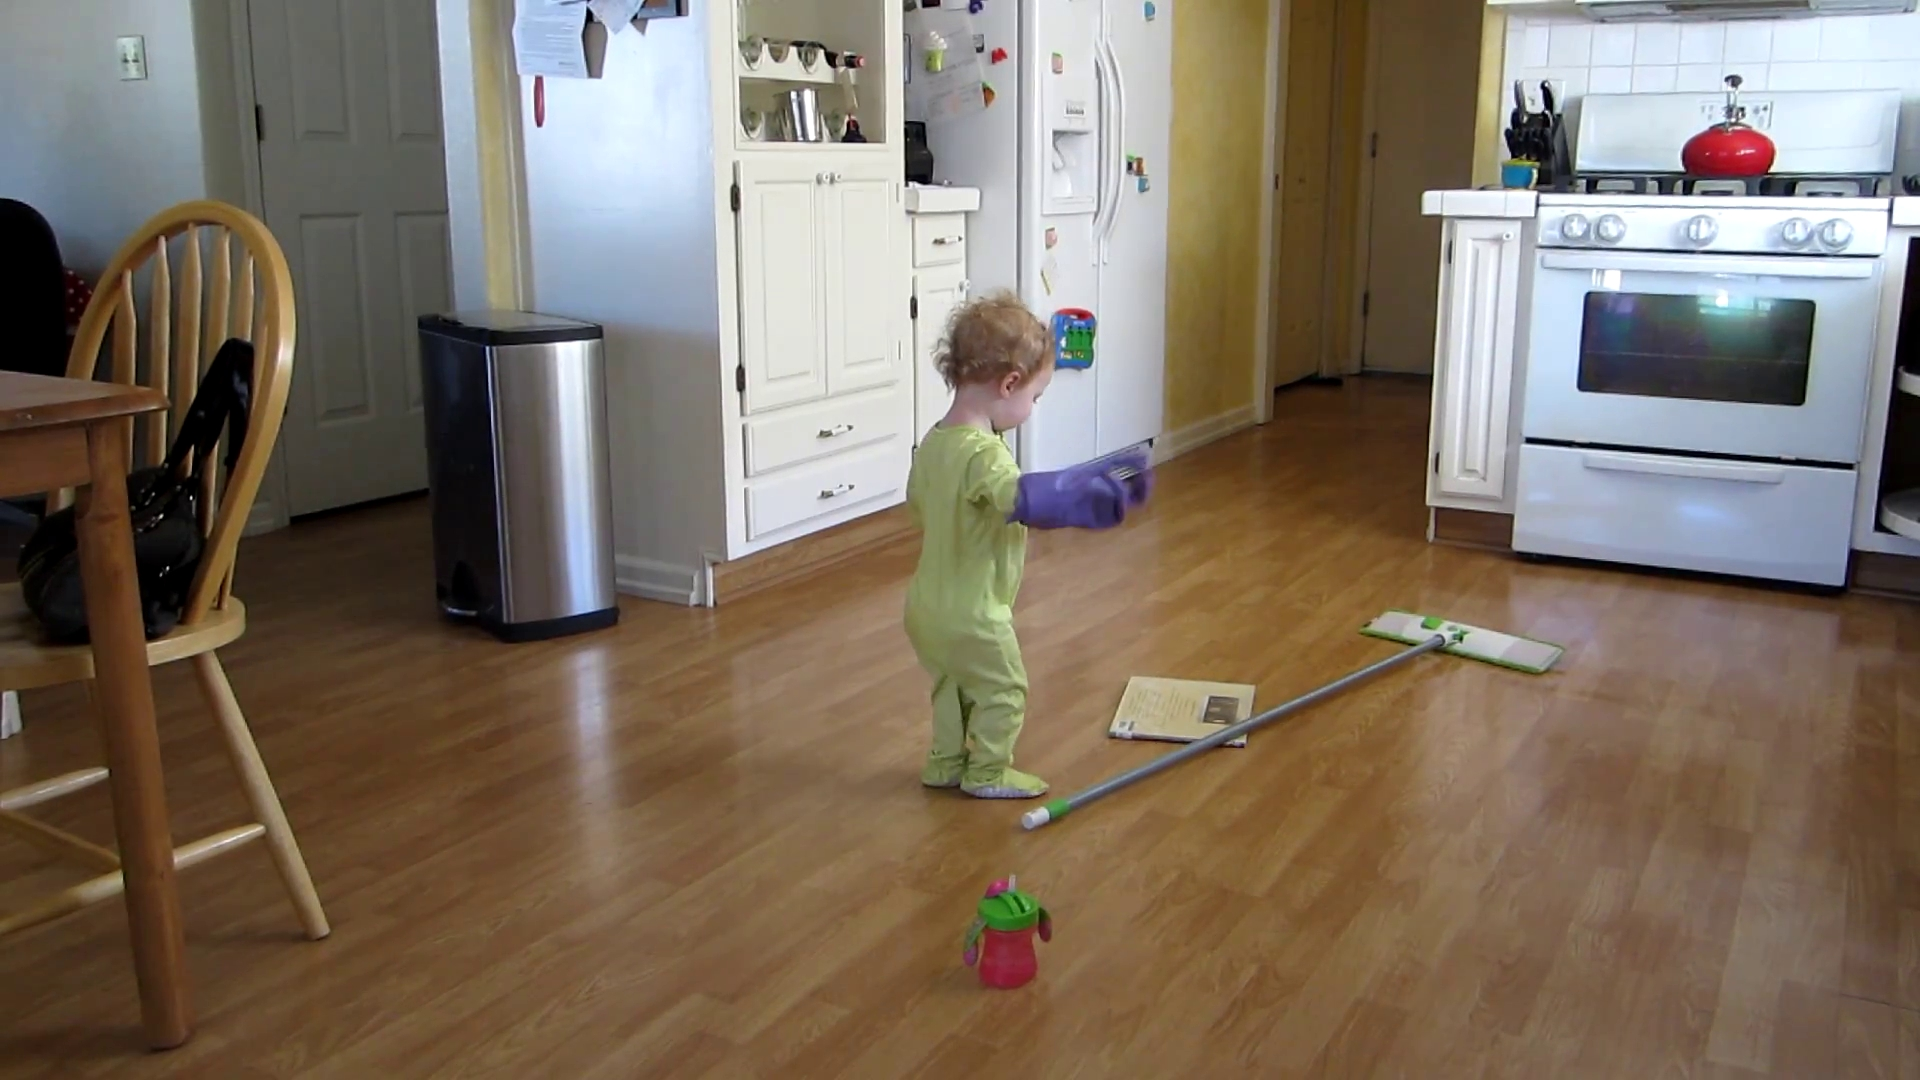
\includegraphics[width=0.8\textwidth]{fig1.jpg}
    \caption{There is a kid.}
    \label{kid}
\end{figure}

\section{Index of Table}
Table~\ref{table1} shows the values of some basic functions.
\begin{table}
    \centering
    \caption{The values of some basic functions.}
    \label{table1}
    \begin{tabular}{l|cccc}
        \hline
        & $x=1$ & $x=2$ & $x=3$ & $x=4$ \\
        \hline
        $y=x$ & 1 & 2 & 3 & 4 \\
        $y=x^{2}$ & 1 & 4 & 9 & 16 \\
        $y=x^{3}$ & 1 & 8 & 27 & 64 \\
        \hline
    \end{tabular}
\end{table}

\end{document}